% This is samplepaper.tex, a sample chapter demonstrating the
% LLNCS macro package for Springer Computer Science proceedings;
% Version 2.20 of 2017/10/04
%
\documentclass[runningheads]{llncs}
%
\usepackage{graphicx}
% Used for displaying a sample figure. If possible, figure files should
% be included in EPS format.
%
% If you use the hyperref package, please uncomment the following line
% to display URLs in blue roman font according to Springer's eBook style:
% \renewcommand\UrlFont{\color{blue}\rmfamily}

\newcommand{\authorname}{Jakob Abfalter} % The author name without titles.
\newcommand{\thesistitle}{Adaptor Signature Based Atomic Swaps Between Bitcoin and a Mimblewimble Based Cryptocurrency} % The title of the thesis. The English version should be used, if it exists.

\newcommand{\styleVariable}[1]{\mathit{#1}}
\newcommand{\styleFunction}[1]{\mathsf{#1}}
\newcommand{\styleCal}[1]{\mathcal{#1}}
\newcommand{\styleSet}[1]{\mathbb{#1}}

% constants
\newcommand{\cnstIntegersPrime}[1]{\ZZ_{#1}}
\newcommand{\cnstIntegersPrimeWithoutZero}[1]{\cnstIntegersPrime{#1}^{*}}
\newcommand{\cnstNatural}{\NN}
\newcommand{\cnstBinary}[1]{\{0,1\}^{#1}}
\newcommand{\cnstEmptySet}{\emptyset}
\newcommand{\cnstHash}{\styleFunction{h}}
\newcommand{\cnstGroup}{\styleSet{G}}
\newcommand{\cnstOracle}{\styleCal{O}}
\newcommand{\cnstRelation}{\styleVariable{R}}
\newcommand{\cnstPolyTime}{\styleVariable{PPT}}
\newcommand{\varG}{\styleVariable{g}}
\newcommand{\varH}{\styleVariable{h}}
\newcommand{\cnstAdversary}{\styleCal{A}}
\newcommand{\cnstaEUFCMA}{\styleFunction{aEUF-CMA}}
\newcommand{\cnstPayToCoin}{\styleVariable{PayToCoin}}
\newcommand{\cnstPayToMuSigCoin}{\styleVariable{PayToMuSigCoin}}
\newcommand{\cnstPayToCoinHideSecret}{\styleVariable{PayToCoinHideSecret}}

% functions
\newcommand{\funHash}[1]{\cnstHash (#1)}
\newcommand{\opPointScalar}[2]{#1^{#2}}
\newcommand{\funGen}[1]{\opPointScalar{\varG}{#1}}
\newcommand{\funGenH}[1]{\opPointScalar{\varH}{#1}}
\newcommand{\funList}[1]{\{#1\}}
\newcommand{\funStar}[1]{#1'}
\newcommand{\funNegl}[1]{\styleFunction{negl}(#1)}

% variables
\newcommand{\varScA}{\styleVariable{a}}
\newcommand{\varScB}{\styleVariable{b}}
\newcommand{\varAlice}{\styleVariable{A}}
\newcommand{\varBob}{\styleVariable{B}}
\newcommand{\varX}{\styleVariable{x}}
\newcommand{\varProbability}{\styleVariable{P}}
\newcommand{\varLanguage}{\styleVariable{L}_\cnstRelation}
\newcommand{\varPrime}{\styleVariable{p}}
\newcommand{\varN}{\styleVariable{n}}
\newcommand{\varTx}{\styleVariable{tx}}
\newcommand{\varTxAlice}{\varTx_{\varAlice}}
\newcommand{\varTxBob}{\varTx_{\varBob}}
\newcommand{\varExcess}{\styleCal{E}}
\newcommand{\varExcessAlice}{\varExcess_{\varAlice}}
\newcommand{\varExcessBob}{\varExcess_{\varBob}}
\newcommand{\varKernel}{\styleVariable{K}}
\newcommand{\varSecKey}{\styleVariable{sk}}
\newcommand{\varSecKeyAlice}{\varSecKey_{\varAlice}}
\newcommand{\varSecKeyBob}{\varSecKey_{\varBob}}
\newcommand{\varSecKeyAdv}{\varSecKey_{\cnstAdversary}}
\newcommand{\varPubKey}{\styleVariable{pk}}
\newcommand{\varPubKeyAlice}{\varPubKey_{\varAlice}}
\newcommand{\varPubKeyBob}{\varPubKey_{\varBob}}
\newcommand{\varPubKeyComp}{\varPubKey_{\styleVariable{comp}}}
\newcommand{\varPubKeyCompApt}{\varPubKey_{\styleVariable{comp\_apt}}}
\newcommand{\varPubKeyAdv}{\varPubKey_{\cnstAdversary}}
\newcommand{\varKeyPair}{(\varSecKey, \varPubKey)}
\newcommand{\varKeyPairAlice}{(\varSecKeyAlice, \varPubKeyAlice)}
\newcommand{\varKeyPairBob}{(\varSecKeyBob, \varPubKeyBob)}
\newcommand{\varSigScheme}{\Phi}
\newcommand{\varSigSchemeMP}{\varSigScheme_{\styleVariable{MP}}}
\newcommand{\varSigSchemeApt}{\varSigScheme_{\styleVariable{Apt}}}
\newcommand{\varProof}{\pi}
\newcommand{\varProofAlice}{\pi_\varAlice}
\newcommand{\varProofBob}{\pi_\varBob}
\newcommand{\varSignature}{\sigma}
\newcommand{\varInput}{\styleVariable{I}}
\newcommand{\varFundValue}{\styleVariable{p}}
\newcommand{\varOffset}{\styleVariable{o}}
\newcommand{\varSupply}{\styleVariable{s}}
\newcommand{\varCoin}{\styleCal{C}}
\newcommand{\varCoinInp}{\varCoin_{\styleVariable{inp}}}
\newcommand{\varCoinOut}{\varCoin_{\styleVariable{out}}}
\newcommand{\varCoinOutAlice}{\varCoinOut^{\varAlice}}
\newcommand{\varCoinOutBob}{\varCoinOut^{\varBob}}
\newcommand{\varCoinSpecial}{\varCoinOut^{\styleVariable{sp}}}
\newcommand{\varValue}{\styleVariable{v}}
\newcommand{\varMsg}{\styleVariable{m}}
\newcommand{\varLockHeight}{\styleVariable{h}}
\newcommand{\varNonce}{\styleVariable{k}}
\newcommand{\varNonceAlice}{\styleVariable{\varNonce_{\varAlice}}}
\newcommand{\varNonceBob}{\styleVariable{\varNonce_{\varBob}}}
\newcommand{\varNonceAdv}{\varNonce_{\cnstAdversary}}
\newcommand{\varBlindingFactor}{\styleVariable{r}}
\newcommand{\varBlindingFactorFor}[1]{\varBlindingFactor_{#1}}
\newcommand{\varS}{\styleVariable{s}}
\newcommand{\varSAlice}{\styleVariable{s}_\varAlice}
\newcommand{\varSBob}{\styleVariable{s}_\varBob}
\newcommand{\varKey}{\styleVariable{x}}
\newcommand{\varKeyVerf}{\varKey_{\styleVariable{p1}}}
\newcommand{\varKeyProv}{\varKey_{\styleVariable{p2}}}
\newcommand{\varKeySt}{\funStar{\varKey}}
\newcommand{\varRand}{\styleVariable{R}}
\newcommand{\varRandAlice}{\varRand_{\varAlice}}
\newcommand{\varRandBob}{\varRand_{\varBob}}
\newcommand{\varRandAdv}{\varRand_{\cnstAdversary}}
\newcommand{\varSigPt}{\widetilde{\varSignature}}
\newcommand{\varSigAlice}{\widetilde{\varSignature_{\varAlice}}}
\newcommand{\varSigAptAlice}{\varSignature^{\varAlice}_{\styleVariable{apt}}}
\newcommand{\varSigAptBob}{\varSignature^{\varBob}_{\styleVariable{apt}}}
\newcommand{\varSigBob}{\widetilde{\varSignature_{\varBob}}}
\newcommand{\varSigPart}{\varSignature_{\styleVariable{prt}}}
\newcommand{\varSigPartAdv}{\varSignature_{\styleVariable{prt}}^{\cnstAdversary}}
\newcommand{\varSigPartSt}{\funStar{\varSignature_{\styleVariable{prt}}}}
\newcommand{\varSchnorrChallenge}{\styleVariable{e}}
\newcommand{\varGSigPart}{\funGen{\varSigPart}}
\newcommand{\varSigPartApt}{\varSignature_{\styleVariable{prt\_apt}}}
\newcommand{\varSigPartAptSt}{\funStar{\varSigPartApt}}
\newcommand{\varGSigPartAptSt}{\funGen{\varSigPartAptSt}}
\newcommand{\varWit}{\styleVariable{x}}
\newcommand{\varGWit}{\styleVariable{X}}
\newcommand{\varStatement}{\styleVariable{X}}
\newcommand{\varSigFin}{\varSignature_{\styleVariable{fin}}}
\newcommand{\varSecParam}{\styleVariable{1^n}}
\newcommand{\varBigA}{\styleVariable{A}}
\newcommand{\varSmallA}{\styleVariable{a}}
\newcommand{\varPublicParam}{\styleVariable{PP}}
\newcommand{\varInputSpace}{\styleSet{I}}
\newcommand{\varRandSpace}{\styleSet{K}}
\newcommand{\varCommitSpace}{\styleSet{C}}
\newcommand{\varCommitment}{\styleVariable{C}}
\newcommand{\varSet}{\styleSet{S}}

% operators
\newcommand{\opAccess}[2]{#1.#2}
\newcommand{\opIn}{\in}
\newcommand{\opNotIn}{\not\opIn}
\newcommand{\opConc}{~||~}
\newcommand{\opForWhich}{~|~}
\newcommand{\opAddScalar}{~+~}
\newcommand{\opAssign}{~:=~}
\newcommand{\opSub}{~-~}
\newcommand{\opNegative}[1]{-#1}
\newcommand{\opTimesScalar}{~\cdot~}
\newcommand{\opAddPoint}{~\cdot~}
\newcommand{\opEq}{~=~}
\newcommand{\opNotEq}{~\neq~}
\newcommand{\opSeperate}{,~}
\newcommand{\opExcluding}{\ensuremath{\setminus}}
\newcommand{\opIff}{~\textit{iff}~}
\newcommand{\opFunResult}{~\leftarrow~}
\newcommand{\opAnd}{~\land~}
\newcommand{\opUnion}{~\cup~}
\newcommand{\opSmEq}{~\leq~}

% procedures
\newcommand{\procGenRId}{\styleFunction{GenR}}
\newcommand{\procGenR}[1]{\procGenRId{#1}}

\newcommand{\procSetupId}{\styleFunction{Setup}}
\newcommand{\procSetup}[1]{\procSetupId(#1)}

\newcommand{\procCommitId}{\styleFunction{Commit}}
\newcommand{\procCommit}[2]{\procCommitId(#1, #2)}
\newcommand{\procSimpleCommitId}{\styleFunction{SimpleCommit}}
\newcommand{\procSimpleCommit}[1]{\procSimpleCommitId(#1)}

\newcommand{\procSignId}{\styleFunction{Sign}}
\newcommand{\procSign}[2]{ \procSignId_{#2}(#1) }
\newcommand{\procVerfId}{\styleFunction{Verf}}
\newcommand{\procVerf}[3]{ \procVerfId_{#3}(#1 \opSeperate #2) }

\newcommand{\procProofId}{\styleFunction{rproof}}
\newcommand{\procProof}[5]{\procProofId_{#4,#5}(#1,#2,#3)}

\newcommand{\procSetupPartSigId}{\styleFunction{setupPt}}
\newcommand{\procSetupPartSig}[1]{\procSetupPartSigId (#1)}
\newcommand{\procGenPartSigId}{\styleFunction{signPt}}
\newcommand{\procGenPartSig}[5]{ \procGenPartSigId_{#2,#3,#4,#5}(#1) }
\newcommand{\procSignPtId}{\styleFunction{signPt}}
\newcommand{\procSignPt}[3]{\procSignPtId<(#1,#2)(#1,#3)>}
\newcommand{\procVerfPtSigId}{\styleFunction{vrfPt}}
\newcommand{\procVerfPtSig}[3]{\procVerfPtSigId(#1,#2,#3)}
\newcommand{\procVerfPartSigId}{\styleFunction{vrfPt}}
\newcommand{\procVerfPartSig}[6]{ \procVerfPartSigId_{#2,#3,#4,#5}(#1 \opSeperate #6) }
\newcommand{\procFinSigId}{\styleFunction{finSig}}
\newcommand{\procFinSig}[2]{ \procFinSigId(#1,#2) }

\newcommand{\procSetupAptId}{\styleFunction{setupApt}}
\newcommand{\procSetupApt}[1]{\procSetupAptId(#1)}
\newcommand{\procGenPtAptSigId}{\styleFunction{signPtPreSig}}
\newcommand{\procGenPtAptSig}[6]{\procGenPtAptSigId_{#2,#3,#4,#5,#6}(#1)}
\newcommand{\procExtWitId}{\styleFunction{extWit}}
\newcommand{\procExtWit}[3]{ \procExtWitId(#1 \opSeperate #2 \opSeperate #3) }
\newcommand{\procVrfAptId}{\styleFunction{vrfPtPreSig}}
\newcommand{\procVrfApt}[7]{ \procVrfAptId_{#2,#3,#4,#5,#6}(#1 \opSeperate #7) }
\newcommand{\procFinAptSigId}{ \styleFunction{finAptPreSig} }
\newcommand{\procFinAptSig}[5]{ \procFinAptSigId_{#3,#4,#5}(#1 \opSeperate #2) }

\newcommand{\procExpForgId}{ \styleFunction{forgeAptSig_{\cnstAdversary}} }
\newcommand{\procExpForg}[1]{ \procExpForgId(#1) }
\newcommand{\procSignOracleId}[2]{ \cnstOracle_{s,#1,#2} }
\newcommand{\procSignOracle}[3]{ \procSignOracleId{#2}{#3}(#1) }
\newcommand{\procFunctionId}{\styleFunction{f}}
\newcommand{\procFunction}[1]{\procFunctionId(#1)}

\newcommand{\procExpExtId}{ \styleFunction{aExtrWit_{\cnstAdversary}} }
\newcommand{\procExpExt}[1]{ \procExpExtId(#1) }
\newcommand{\procNonceOracleId}{ \cnstOracle_{k}}
\newcommand{\procNonceOracle}[1]{ \procNonceOracleId(#1) }
\newcommand{\procSignPtOracleId}[2]{ \cnstOracle_{s,#1,#2} }
\newcommand{\procSignPtOracle}[3]{ \procSignPtOracleId{#2}{#3}(#1) }

\newcommand{\procCreatePreTxId}{ \styleFunction{createPreTx} }
\newcommand{\procCreatePreTx}[6]{ \procCreatePreTxId_{#2,#3,#4,#5,#6}(#1) }
\newcommand{\procRecvTxId}{ \styleFunction{recvTx} }
\newcommand{\procRecvTx}[4]{ \procRecvTxId_{#3,#4}(#1,#2) }
\newcommand{\procFinalizeTxId}{ \styleFunction{finalizeTx} }
\newcommand{\procFinalizeTx}[2]{ \procFinalizeTxId_{#1}(#2) }
\newcommand{\procSpendOutputId}{ \styleFunction{spendTxOutput} }


\usepackage{varwidth}
\usepackage[
    n,
    advantage,
    operators,
    sets,
    adversary,
    landau,
    probability,
    notions,
    logic,
    ff,
    mm,
    primitives,
    events,
    complexity,
    asymptotics,
    keys
]{cryptocode}

\begin{document}
%
\title{Title here\thanks{Supported by organization x.}}
%
%\titlerunning{Abbreviated paper title}
% If the paper title is too long for the running head, you can set
% an abbreviated paper title here
%
\author{First Author\inst{1}\orcidID{0000-1111-2222-3333} \and
Second Author\inst{2,3}\orcidID{1111-2222-3333-4444} \and
Third Author\inst{3}\orcidID{2222--3333-4444-5555}}
%
\authorrunning{F. Author et al.}
% First names are abbreviated in the running head.
% If there are more than two authors, 'et al.' is used.
%
\institute{Princeton University, Princeton NJ 08544, USA \and
Springer Heidelberg, Tiergartenstr. 17, 69121 Heidelberg, Germany
\email{lncs@springer.com}\\
\url{http://www.springer.com/gp/computer-science/lncs} \and
ABC Institute, Rupert-Karls-University Heidelberg, Heidelberg, Germany\\
\email{\{abc,lncs\}@uni-heidelberg.de}}
%
\maketitle              % typeset the header of the contribution
%
\begin{abstract}
The abstract should briefly summarize the contents of the paper in
150--250 words.

\keywords{First keyword  \and Second keyword \and Another keyword.}
\end{abstract}


\todo[inline]{Pedro: Although not strictly required, IMO it is nice to have some text here introducing what the reader should expect in the rest of the section. For instance: \\
In this section, we first introduce the notation and definitions used hereby in this thesis. Then, we ...... Finally, we introduce.....}

\section{General Notation and Definitions}\label{sec:generalNotationDefinitions}




\paragraph{Notation}
We first define the general notation used in the following chapters to formalize procedures and protocols. Let $\cnstGroup$ denote a cyclic group of prime order $\varPrime$ and $\cnstIntegersPrime{\varPrime}$
the ring of integers modulo $\varPrime$ with identity element $\cnstIdentityElement$. $\cnstIntegersPrimeWithoutZero{\varPrime}$ is $\cnstIntegersPrime{\varPrime} \opExcluding \funList{0}$. \todo{Pedro: I think macro $\opExcluding$ was broken here. I have updated to use $\setminus$ instead. Please check that this is what you expected} $\varG \opSeperate \varH$ are adjacent
generators in $\cnstGroup$, where adjacent means the discrete logarithm of $\varH$ in regards to $\varG$ is not known. Exponentiation stands for repeated application of the group operation. We define the group operation between two curve points as
$\funGen{\varScA} \opAddPoint \funGen{\funGen{\varScB}} \opEq \funGen{\varScA \opAddScalar \varScB}$.

\todo{Pedro: We normally do not use the tilde to add spaces in math mode}

\begin{definition}[Hard Relation\cite{aumayr2020bitcoinchannels}]\label{def:hardRelation}
    Given a language $\varLanguage \opAssign \funList{\varBigA \opForWhich \exists\varSmallA \text{ s.t. } (\varBigA, \varSmallA) \opIn \cnstRelation}$ then the relation $\cnstRelation$ is
    considered hard if the following three properties hold:
    \begin{enumerate}
        \item $\procGenR{(\varSecParam)}$ is a $\cnstPolyTime$ sampling algorithm which outputs a statement/witness of the form $(\varBigA, \varSmallA) \opIn \cnstRelation$.
        \item Relation $\cnstRelation$ is poly-time decidable.
        \item For all $\cnstPolyTime$ adversaries $\cnstAdversary$ the probability of finding $\varSmallA$ given $\varBigA$ is negligible.
    \end{enumerate}
    
    
    \todo[inline]{Pedro: I would include these two relations below as your own definitions because I imagine that you would like to refer to them afterwards in the thesis} 
    In this thesis we find two types of hard relations:
    \begin{enumerate}
        \item The output of a secure hash function (as defined in~\ref{def:hashFunction}) and it's input $(\varInput, \funHash{\varInput})$.
        \item The discrete logarithm $\varX$ of $\funGen{\varX}$ in the group $\cnstGroup$.
    \end{enumerate}
\end{definition}


\todo[inline]{Pedro: Link to paper/book where you got this definition from is missing}
\begin{definition}[Signature Scheme]\label{def:signatureScheme}
    A valid \todo{Pedro: What is valid here? You have not defined it before} Signature Scheme must provide three procedures: \todo[inline]{Pedro: I would write this sentence as: A signature scheme $\varSigScheme$ is a tuple of algorithms $(\procSetupId \opSeperate \procSignId \opSeperate \procVerfId)$ defined as follows: }
    \[ \varSigScheme = (\procSetupId \opSeperate \procSignId \opSeperate \procVerfId) \]
    
    \todo[inline]{Pedro: write the API of the algorithms in bullet points} 
    $(\varSecKey, \varPubKey) \gets \procSetup{\varSecParam}$ takes as input a security parameter $\varSecParam$ and outputs a keypair $\varKeyPair$, consisting of a secret key $\varSecKey$ and a public key $\varPubKey$, whereas
    the secret key has to be kept private and the public key is shared with other parties.
    $\varSecKey$ can be used together with a message $\varMsg$ to call the $\procSign{\varSecKey}{\varMsg}$ procedure to create a signature $\varSignature$ over the message $\varMsg$.
    Parties knowing $\varPubKey$ can then test the validity of the signature by calling $\procVerf{\varPubKey}{\varSignature}{\varMsg}$ with the same message $\varMsg$. The procedure will only output $1$ if the message was
    indeed signed with the correct secret key $\varSecKey$ of $\varPubKey$ and therefore proves the possesion of $\varSecKey$ by the signer \todo{Pedro: ``proving that the sender had the $\varSecKey$'' is a property that no all signature schemes may have}.
    A valid signature scheme have to fulfill two security properties
    \todo[inline]{Pedro:  Choose one unforgeability form, the one that you require later in the thesis}
    \begin{itemize}
        \item Correctness: For all messages $\varMsg$ and valid keypairs $\varKeyPair$ the following must hold $\procVerf{\varPubKey}{\procSign{\varSecKey}{\varMsg}}{\varMsg} \opEq 1$ \todo{Pedro: Except with negligible probability}
        \item Unforgeability: Note that there are different levels of Unforgability:~\cite{goldwasser1988digital}
        \begin{itemize}
            \item Universal Forgery: The ability to forge signatures for any message.
            \item Selective Forgery: The ability to fogre signatures for messages of the adversary's choice.
            \item Existential Forgery: The ability to forge a valid signature / message pair not previously known to the adversary.
        \end{itemize}
    \end{itemize}
\end{definition}

\todo[inline]{Pedro: nice that you have defined the three properties. I would keep the one that you need later}

\begin{definition}[Cryptographic Hash Function]\label{def:hashFunction}
    A cryptographic hash function $\cnstHash$\todo{Pedro: minor thing: we normally use capital H} is defined as $\funHash{\varInput} \rightarrow \cnstBinary{\varN}$ for some fixed number $\varN$ and some input $\varInput$. A secure hashing function
    has to fullfill the following security properties:~\cite{al2011cryptographic}
    \begin{itemize}
        \item Collision-Resistence (CR): Collision-Resistance means that it is computationally infeasible to find two inputs $\varInput_1$ and $\varInput_2$ such that
        $\funHash{\varInput_1} \opAssign \funHash{\varInput_2}$ with $\varInput_1 \opNotEq \varInput_2$.
        \item Pre-image Resistence (Pre): In a hash function $\cnstHash$ that fulfills Pre-image Resistance it is infeasible to recover the original input $\varInput$ from its hash output $\funHash{\varInput}$.
        If this security property is achieved, the hash function is said to be non-invertible.
        \item 2nd Pre-image Resistence (Sec):  This property is similar to Collision-Resistance and is sometimes referred to as \textit{Weak Collision-Resistance}.
        Given such a hash function $\cnstHash$ and an input $\varInput$, it should be infeasible to find a different input $\funStar{\varInput}$ such that $\varInput \opNotEq \funStar{\varInput}$
        and $\funHash{\varInput} \opEq \funHash{\funStar{\varInput}}$.
    \end{itemize}
\end{definition}


\todo[inline]{Pedro: I think here the Open operation of the commitment is missing, which you need later for the binding property}
\begin{definition}[Commitment Scheme~\cite{bunz2018bulletproofs}]\label{def:commitment}
    A cryptographic Commitment Scheme $\varCommitScheme$ is defined by a pair of functions $(\procSetup{\varSecParam} \opSeperate \procCommitId(\varInput, \varNonce))$. $\procSetupId$ is the setup procedure, it takes as input a
    security parameter $\varSecParam$ and outputs public parameters $\varPublicParam$. Depending on $\varPublicParam$ we define a input space $\varInputSpace_{\varPublicParam}$,
    a randomness space $\varRandSpace_{\varPublicParam}$ and a commitment space $\varCommitSpace_{\varPublicParam}$.

    The function $\procCommitId$ takes an arbitrary input $\varInput \opIn \varInputSpace_{\varPublicParam}$, and a random value $\varNonce \opIn \varRandSpace_{\varPublicParam}$ and
    generates an output$\varCommitment \opIn \varCommitSpace_{\varPublicParam}$.

    Secure commitments must fullfill the \textit{Binding} and \textit{Hiding} security properties:
    \begin{itemize}
        \item \textit{Binding:} If a Commitment Scheme is binding it must hold that for all $\cnstPolyTime$ adversaries $\cnstAdversary$ given a valid input $\varInput \opIn \varInputSpace_{\varPublicParam}$
        and randomness $\varNonce \opIn \varRandSpace_{\varPublicParam}$ the probabilty of finding a $\funStar{\varInput} \opNotEq \varInput$ and a $\funStar{\varNonce}$ with
        $\procCommit{\varInput}{\varNonce} \opEq \procCommit{\funStar{\varInput}}{\funStar{\varNonce}}$ is negligible.
        \item \textit{Hiding:} For a $\cnstPolyTime$ adversary $\cnstAdversary$, commitment inputs $\varInput \opIn \varInputSpace_{\varPublicParam} \opSeperate \varNonce \opIn
       \varRandSpace_{\varPublicParam}$ and a commitment output $\varCommitment \opAssign \procCommit{\varInput, \varNonce}$ the probabilty of the adversary choosing the correct input
        $\funList{\varInput, \funStar{\varInput}}$ must not be higher then $\frac{1}{2} + \funNegl{\varProbability}$. \todo{Pedro: this definition  seems wrong to me? Where does $\funStar{\varInput}$ come from?}
    \end{itemize}
\end{definition}

\todo[inline]{Pedro: Add reference from where you took this definition. You may want to add that it is an ``Additive'' Homomorphic Commitment}
\begin{definition}[Homomorphic Commitment]\label{def:homomorphicCom}
    If a Commitment Scheme as defined in~\ref{def:commitment} is homomorphic then the following must hold
    \[ \procCommit{\varInput_1}{\varNonce_1} \opAddPoint \procCommit{\varInput_2}{\varNonce_2} \opEq \procCommit{\varInput_1 \opAddScalar \varInput_2}{\varNonce_1 \opAddScalar \varNonce_2} \]
\end{definition}

\todo[inline]{First, a Pedersen Commitment is an instance of Commitment Scheme as in Def 3.4; Second it has the homomorphic property as in 3.5. Clarify that, for instance, by explaining exactly how the algorithms are implemented, as you did below.}
\begin{definition}[Pedersen Commitment]\label{def:pedersenCom}
    A Pedersen Commitment is an instantiation of a Homomoprhic Commitment Scheme as defined in~\ref{def:homomorphicCom}:
    \[ \varCommitSpace_{\varPublicParam} \opAssign \cnstGroup\] of order $\varPrime \opSeperate \varInputSpace_{\varPublicParam} \opSeperate \varRandSpace_{\varPublicParam} \opAssign \cnstIntegersPrime{\varPrime}$.
    the procedures $(\procSetupId, \procCommitId)$ are then instantiated as:
    \[ \procSetup{\varSecParam} \opAssign \varG, \varH \sample \cnstGroup\]
    \[ \procCommit{\varInput}{\varNonce} \opAssign \funGen{\varNonce} \funGenH{\varInput} \]

\end{definition}


\section{Bitcoin}\label{sec:bitcoin}

In this section we will discuss the basics of the Bitcoin transaction protocol.
We will find definitions which we will use later in section~\ref{sec:atomic-swap} to construct an atomic swap protocol.
The main reference of this section is the book Mastering Bitcoin by Andreas Antonopoulos~\cite{antonopoulos2014mastering}.

\subsection{Bitcoin Transaction Protocol}\label{subsec:bitcointx}

A \emph{Bitcoin Transaction} is a data structure which allows transferring value between participants of the network.
In Bitcoin there are no user balances or user accounts, instead the UTXO model (unspent transaction outputs) is empoloyed.
An UTXO is a output constructed in a previous transaction which holds value in the form of an amount expressed in
Bitcoin (more precisely in Satoshis, which is the smallest unit of Bitcoin) and a locking condition (referred to as
scriptPubKey).
Unspent means that this output has not been spent yet in a transaction and its funds are therefore available to be redeemed by a participant capable of unlocking the output.
To unlock this value one has to provide a script fulfilling the locking condition, referred to as scriptSig.
In the most common case the lock condition will be to provide a valid signature under a public key.
This is referred to as a P2PK or P2PKH output which we will see in more detail in section~\ref{subsubsec:p2pk}.
However, more complex conditions, such we shall see in section~\ref{subsubsec:p2sh} are possible.

\begin{definition}[Unspent Transaction Output - UTXO] An unspent transaction output is a data structure
consisting of a locking condition $\varScriptPubKey$, a value expressed in Bitcoin $\varValue$ and an unlocking script $\varScriptSig$ which is
initially empty and has to be provided by the owner when spending the UTXO in a transaction. In this paper we
generally use $\varUTXO$ to refer to a singular UTXO and $\varUTXOSet$ to refer to a set of UTXOs.
    \[ \varUTXO \opAssign \{ \varValue \opSeperate \varScriptPubKey \opSeperate \varScriptSig \} \]
\end{definition}

We define three auxiliary functions for the creation, spending and verification of an UTXO.
Note that we use $\procVerfId$ as a generalization of a verification function.
In practice verifcation of a UTXO will most of the time correspond to the verification of a digital signature.
However, as we shall see in~\ref{subsubsec:p2sh} this is not necessarily always the case.

\begin{center}
    \fbox{
    \begin{varwidth}{\textwidth}
        \procedure[linenumbering]{$\procCreateUTXO{\varValue}{\varScriptPubKey}$} {
        \pcreturn \varUTXO \opAssign \{ \varValue \opAssign \varValue, \varScriptPubKey \opAssign \varScriptPubKey,
        \varScriptSig \opAssign \cnstEmptySet \}
        } \\
        \procedure[linenumbering]{$\procSpendUTXO{\varUTXO}{\varScriptSig}$} {
        \{ \varValue, \varScriptPubKey \} \opFunResult \varUTXO \\
        \pcreturn \varUTXO \opAssign \{ \varValue \opAssign \varValue, \varScriptPubKey \opAssign \varScriptPubKey,
        \varScriptSig \opAssign \varScriptSig \}
        } \\
        \procedure[linenumbering]{$\procVerfUTXO{\varUTXO}$} {
        \{ \varValue, \varScriptPubKey, \varScriptSig \} \opFunResult \varUTXO \\
        \pcreturn \procVerf{\varScriptPubKey}{\varScriptSig}{\varValue}
        }
    \end{varwidth}
    }
\end{center}

Now a full transaction consists of one, or many UTXOs as inputs and one or many UTXOs as output.
For the transaction to be considered valid the $\varScriptSig$ fields in the inputs need the be correctly filled, and the value in the newly created output UTXOs must not exceed the value stored in the spending UTXOs.
A value lower than what is provided in the inputs is allowed, this means the miner of the transaction gets to collect the difference as a fee.
The higher this fee, the more incentive the miners will have to include your transaction in the blockchain.
Additionally a transaction consists of a version number, and a locktime field which semantically means that a
transaction will only be seen as valid after a certain block number in the Bitcoin blockchain was mined.
Figure~\ref{fig:btc-tx} shows a decoded Bitcoin transaction.

\begin{definition}[Bitcoin Transaction]
    A Bitcoin transaction consists of a series of input UTXOs $\varBtcInputs$, a series of output UTXOs $\varBtcOutpus$, a
    transaction version $\varVersion$, and an optional locktime $\varTime$:
    \[ \varBtcTx \opAssign \{ \varVersion, \varTime, \varBtcInputs, \varBtcOutpus \} \]
\end{definition}

\begin{figure}
    \begin{center}
        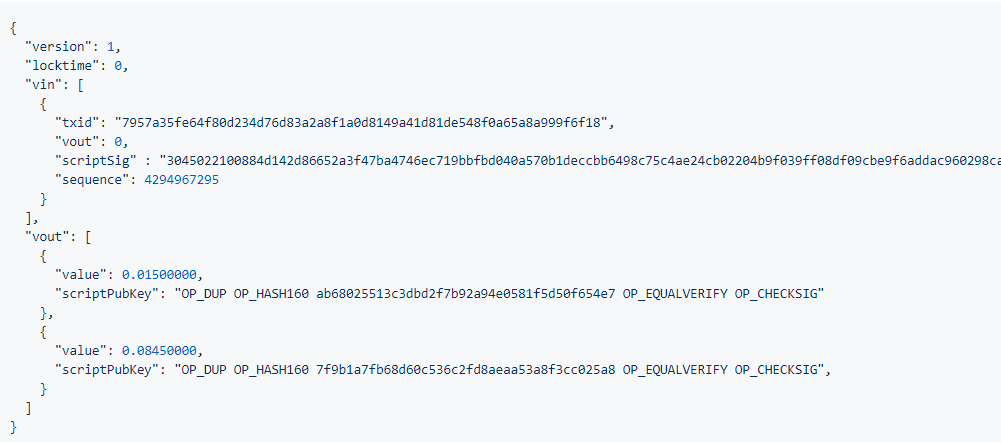
\includegraphics[width=\textwidth]{btc-tx.png}
    \end{center}
    \caption{A decoded Bitcoin transaction~\footcite{https://github.com/bitcoinbook/bitcoinbook/blob/develop/ch06.asciidoc} \label{fig:btc-tx}}
\end{figure}

A transaction is valid if the follwing conditions are fullfilled:

\begin{itemize}
    \item The total value of inputs is greater or equal the total value of outputs.
    \item For all $\varUTXO \opIn \varUTXO$ $\procVerfUTXO{\varUTXO} \opEqNoQ 1$ must hold.
    \item All input UTXOs have not been spent before.
    \item If a locktime $\varTime$ is given, the current block on the Bitcoin blockchain needs to be higher or equal $\varTime$.
\end{itemize}

\begin{definition}[Bitcoin Transaction Scheme]
    We define a Bitcoin Transaction scheme as a tupel of three DPT functions $(\procBuildTransactionId,
    \procSignTransactionId, \procVerfTransactionId)$.
    \begin{itemize}
        \item $\varBtcTx \opFunResult \procBuildTransaction{\varBtcInputs}{\varBtcOutpus}{\varVersion}{\varTime}$: The
        transaction building algorithm is a DPT function which takes as input a set of unspent transaction outputs
        $\varBtcInputs$, a set of newly created transaction outputs $\varBtcOutpus$ a version number $\varVersion$
        and a optional locking time $\varTime$. The algoritm will output an unsigned transaction $\varBtcTx$.
        \item $\funStar{\varBtcTx} \opFunResult \procSign{\varBtcTx}{\funArray{\varScriptSig}}$: The transaction
        signing algoritm is DPT function which takes as input a unsigned Bitcoin transaction $\varBtcTx$ and an array
        of unlocking scripts $\funArray{\varScriptSig}$ for all inputs of the transaction. The algoritm outputs a
        signed Bitcoin transaction which can now be broadcast to the network.
        \item $\{ 1,0 \} \opFunResult \procVerfTransaction{\varBtcTx}$: The verification algorithm is a DPT function
        taking as input a transaction $\varBtcTx$ outputing 1 on a successfull verification or 0 otherwise. The
        function will check the well-balancedness of the transaction, verify the unlocking scripts, locktime
        as well as scanning through the blockchain if all inputs are indeed unspent.
        Note that any public verifier with access to the blockchain ledger and $\varBtcTx$ will be able to perform the verification.
    \end{itemize}
\end{definition}

Following we will outline two common structures of Bitcoin outputs the P2PK/P2PKH and the P2SH outputs.

\subsubsection{P2PK, P2PKH\label{subsubsec:p2pk}}

P2PK stands for Pay-to-Public-Key and P2PKH for Pay-to-Public-Key-Hash.
In this type of output $\varScriptPubKey$ will be constructed such that its value unlocks if a correct signature is
provided in $\varScriptSig$ for a corresponding public key $\varPubKey$.
P2PKH is an update to this script in which the $\varScriptPubKey$ contains a hashed version of the public key $\varPubKey$,
instead of the public key itself.
To spend a P2PKH output one has to provide the unhashed public key in addition to a valid signature.
This type of output, is the most commonly used output in the Bitcoin blockchain to transfer value from one participant to another.
Delgado et at. found in their paper Analysis of the Bitcoin UTXO set from 2017 that more then 80\% of the UTXO set at
that time consisted of P2PKH transactions, whereas about 17\% were P2SH and 0.12\% P2PK outputs.
~\cite{delgado2018analysis}
P2PKH outputs can be encoded into a Bitcoin address using base58 encoding.
This addresses can be handed out to request a payment from somebody.

\subsubsection{P2SH\label{subsubsec:p2sh}}

If more advanced spending conditions, such as multi signature are required, P2SH (Pay-to-script-hash), introduced in
2012, is a way to implement those in a space efficient and simple matter.
Here the locking condition $\varScriptPubKey$ does not contain a script, but instead the hash of a script.
Upon spending the spender has to provide the original script as well as the unlocking requirements for the script
itself.
Upon verification the hash of the provided script will be computed and compared with the value given in the locking
condition, if those match the actual script will be executed.
The advantages of using this approach over just handcrafting a custom locking script is that the locking scripts are
rather short making the transactions smaller and therefore reducing fees, or rather shifting the fees from the sender
to the owner of the output.
Additionally this type of output can be encoded again into a Bitcoin address similar to a P2PKH output, making it
easy to request a payment.

\subsection{Bitcoin Scaling and Layer Two Solutions}\label{sec:bitcoinScaling}

\section{Privacy-enhancing Cryptocurrencies}\label{sec:privacyCryptos}

\subsection{Zero Knowledge Proofs}\label{sec:zeroKnowlegde}

\subsection{Range Proofs}\label{sec:rangeProof}

\begin{definition}[Rangeproof System]
    A Rangeproofs system $\varRProofSystemParam{\varCommitScheme}$ with regards to a homomorphic commitment scheme $\varCommitScheme$ consists of a tupel of functions $(\procRProofSetupId, \procProofId, \procVerfProofId)$.
    \begin{itemize}
        \item $(\varLowerBound,\varUpperBound) \opFunResult \procRProofSetup{\varSecParam}{\varI}{\varJ}$: The rangeproof setup algorithm takes as input a security paramter $\varSecParam$ as well as two numbers
        $\varI$ and $\varJ$ which are treated as exponents of 2 to define the lower and upper bound of the rangeproof protocol.
        \item $\varProof \opFunResult \procProof{\varCommitment}{\varValue}{\varBlindingFactor}$: The proof algorithm is a DPT function which takes as input a commitment $\varCommitment$ a value $\varValue$ and
        a blinding factor $\varBlindingFactor$. It will output a proof $\varProof$ attesting to the statement that the value $\varValue$ of commitment $\varCommitment$ is in between the range $\langle \varLowerBound, \varUpperBound \rangle$ as
        defined during the $\procRProofSetupId$ function.
        \item $\{1,0\} \opFunResult \procVerfProof{\varProof}{\varCommitment}$: The proof verification algorithm is a DPT function which verifies the validity of the proof $\varProof$ with regards to the commitment
        $\varCommitment$. It will output 1 upon a successfull verification or 0 otherwise.
    \end{itemize}
\end{definition}

\begin{definition}[Multiparty Rangeproof System]
    A Multiparty Rangeproof Sytem $\varMPRProofSystemParam{\varCommitScheme}$ with regards to a homomorphic commitment scheme $\varCommitScheme$ is an extension of the regular Rangeproof Sytem with the following
    distributed protocol $\procDRProofId$.
    \begin{itemize}
        \item $\varProof \opFunResult \procDRProof{\varCommitment}{\varValue}{\varBlindingFactorAlice}{\varBlindingFactorBob}$: The distributed proof protocol allows two parties Alice and Bob, each owning a share of the
        commitment $\varCommitment$ to cooperate in order to produce a valid range proof $\varProof$ without a party learning the blinding factor share from the other party.
    \end{itemize}
\end{definition}

For MP proofs \cite{klinec2020privacy}

\subsection{Mimblewimble}\label{sec:Mimblewimble}
In this section we will outline the fundamental properties of the protocols employed in Mimblewimble which are relevant for the thesis and particularily the construction of the Atomic Swap protocol defined in
\ref{chp:atomicSwap}.
\subsubsection{Transaction Structure}
\todo[inline]{Pedro: I think that throughout this section, you have nice explanations of the different parts of the transaction. It would be also possible to add definitions for the different things that you use}

\begin{itemize}
    \item For two adjacent elliptic curve generators $\varG$ and $\varH$ a coin in Mimblewimble is a tuple of the form ($\varCoin$, $\varProof$), where $\varCoin \opAssign \funGen{\varValue} \opAddPoint \funGenH{\varNonce}$  a Pedersen Commitment~\cite{pedersen1991non}
    to the value $\varValue$ with blinding factor $\varNonce$. $\varProof$ is a range proof attesting to the statement that $\varValue$ is in a valid range \todo{Pedro: you might want to specify what range is used here. Also I rewrote some part, so please check.} in zero-knowledge.
    
    \todo[inline]{Pedro: not sure whether the point below is required}
    \item As already pointed out, there are now addresses in Mimblewimble. Ownership of a coin is equivalent to the knowledge of its opening, so the blinding factor takes the role of the secret key.
    
    \item A transaction consists of $\varCoinInp \opAssign (\varCoin_1 \opSeperate \dots \opSeperate \varCoin_n)$ input coins and $\varCoinOut \opAssign (\varCoin'_1 \opSeperate \dots \opSeperate \varCoin'_n)$ output coins.
\end{itemize}
A transaction is considered valid iff $\sum{\varValue'_i} \opSub \sum{\varValue_i} \opEq 0$ so the sum of all input values has to be 0. (Not taking transaction fees into account) \todo[inline]{Pedro: doesn't need to check the range proofs as well?}
From that we can derive the following equation:
\[ \sum{\varCoinOut} \opSub \sum{\varCoinInp} \opAssign \sum{(\funGenH{\varValue'_i} \opAddPoint \funGen{\varNonce'_i})} \opSub \sum{(\funGenH{\varValue_i} \opAddPoint \funGen{\varNonce_i})} \]
So if we assume that a transaction is valid then we are left with the following so called excess value:
\[ \varExcess \opAssign \funGen{(\sum{\varNonce'_i} \opSub \sum{\varNonce_i})} \]
Knowledge of the opening of all coins and the validity of the transaction implies knowledge of $\varExcess$. \todo{Pedro: You mean knowledge of the exponent of $\varExcess$?} 
Directly revealing the opening to $\varExcess$ would leak too much information, an adversary knowing the openings for input coins and all but one output coin, could easily calculate the unknown opening given $\varExcess$.
Therefore knowledge of $\varExcess$ instead is proven by providing a valid signature for $\varExcess$ as public key.
Coinbase transactions (transactions creating new money as part of a miners reward) additionally include the newly minted money as supply $\varSupply$ in the excess equation:
\[ \varExcess \opAssign \funGen{(\sum{\varNonce'_i} \opSub \sum{\varNonce_i})} \opSub \funGenH{\varSupply} \]
Finally a Mimblewimble transaction is of form:
\[ \varTx \opAssign (\varSupply \opSeperate \varCoinInp \opSeperate \varCoinOut \opSeperate \varKernel)\:\text{with}\:\varKernel \opAssign (\funList{\varProof} \opSeperate \funList{\varExcess} \opSeperate \funList{\varSignature}) \]
where $\varSupply$ is the transaction supply amount, $\varCoinInp$ is the list of input coins, $\varCoinOut$ is the list of output coins and $\varKernel$ is the transaction Kernel. The Kernel consists of $\funList{\varProof}$
which is a list of all output coin range proofs, $\funList{\varExcess}$ a list of excess values and finally $\funList{\varSignature}$ a list of signatures ~\cite{fuchsbauer2019aggregate}. \todo{Pedro: the $\varExcess$ is a single value? or a set?}

\subsubsection{Transaction Merging}
An essential property of the Mimblewimble protocol is that two transactions can easily be merged into one, which is essentially a non-interactive version of the CoinJoin protocol on Bitcoin~\cite{maxwell2013coinjoin}
Assume we have the following two transactions:
\[ \varTx_0 \opAssign (\varSupply_0 \opSeperate \varCoinInp^0 \opSeperate \varCoinOut^0 \opSeperate (\funList{\varProof_0} \opSeperate \funList{\varExcess_0} \opSeperate \funList{\varSignature_0}) ) \]
\[ \varTx_1 \opAssign (\varSupply_1 \opSeperate \varCoinInp^1 \opSeperate \varCoinOut^1 \opSeperate (\funList{\varProof_1} \opSeperate \funList{\varExcess_1} \opSeperate \funList{\varSignature_1}) ) \]
Then we can build a single merged transaction:
\[ \varTx_m \opAssign (\varSupply_0 \opAddScalar \varSupply_1 \opSeperate \varCoinInp^0 \opConc \varCoinInp^1,\:\varCoinOut^0 \opConc \varCoinOut^1 \opSeperate (\funList{\varProof_0} \opConc \funList{\varProof_1}) \opSeperate
\funList{\varExcess_0} \opConc \funList{\varExcess_1} \opSeperate \funList{\varSignature_0} \opConc \funList{\varSignature_1}) \]
We can easily deduce that if $\varTx_0$ and $\varTx_1$ are valid, it follows that $\varTx_m$ also has to be valid:
If $\varTx_0$ and $\varTx_1$ are valid that means $\varCoinInp^0 \opSub \varCoinOut^0 \opSub \funGenH{\varSupply_0} \opAssign \varExcess_0 \opSeperate \funList{\varProof_0}$ contains valid range proofs for the outputs
$\varCoinOut^0$ and $\funList{\varSignature_0}$ contains a valid signature to $\varExcess_0 \opSub \funGenH{\varSupply_0}$ as public key, the same must hold for $\varTx_1$.

By the rules of arithmetic it then must also hold that
\[ \varCoinInp^0 \opConc \varCoinInp^1 \opSub \varCoinOut^0 \opConc \varCoinOut^1 \opSub \funGenH{\varSupply_0 \opAddScalar \varSupply_1} \opAssign \varExcess_0 \opAddPoint \varExcess_1 \opSeperate \funList{\varProof_0} \opConc \funList{\varProof_1} \]
must contain valid range proofs for the output coins and $\funList{\varSignature_0} \opConc \funList{\varSignature_1}$ must contain valid signatures to the respective Excess points, which makes $\varTx_m$ a valid transaction.

\subsubsection{Subset Problem}
\todo[inline]{Pedro: I think the content below is not fully clear yet. If needed for the rest, we need to clarify (e.g., add an example?)}
A subtle problem arises with the way transactions are merged in Mimblewimble. From the shown construction, it is possible to reconstruct the original separate transactions from the merged one,
which can be a privacy issue. Given a set of inputs, outputs, and kernels, a subset of these will recombine to reconstruct one of the valid transaction which were aggregated since Kernel Excess values are not combined.
(which would invalidate the signatures and therefore break the security of the system) This problem has been mitigated in Cryptocurrencies implementing the protocol by including an
additional variable in the Kernel, called offset value. The offset is randomly chosen and needs to be added back to the Excess values to verify the sum of the commitments to zero.
\[ \sum{\varCoinOut} \opSub \sum\varCoinInp \opSub \funGenH{\varSupply} \opAssign \opPointScalar{\varExcess}{\varOffset} \]
Every time two transactions are merged, the offset values are combined into a single value. If offsets are picked truly randomly, and the possible range of values is broad enough, the probability of recovering the
uncombined offsets from a merged one becomes negligible, making it infeasable to recover original transactions from a merged one~\cite{poelstra2016mimblewimble}.



\subsubsection{Cut Through}
\todo{Pedro: This requires further explanation and maybe an example?}
From the way transactions are merged together, we can now learn how to purge spent outputs securely. Let's assume $\varCoin_i$ appears as an output in $\varTx_0$ and as an input in $\varTx_1$,
which are being merged. Remembering the equation for transaction balancedness, $\varCoinInp \opSub \varCoinOut \opAssign \varExcess$ if $\varCoin_i$ appears both in the inputs and outputs, and we erase it on both sides, the equation will still hold.
Therefore every time a transaction spends an output, it can be virtually forgotten to improve transaction unlinkability as well as yielding saving space.

\subsubsection{The Ledger}
\todo[inline]{Pedro: Do we need this subsection?}
The ledger of the Mimblewimble protocol itself is a transaction of the already discussed form. Initially, the ledger starts empty, and transactions are added and aggregated recursively.
\begin{itemize}
    \item Only transactions in which input coins are contained in the output coins of the ledger will be valid.
    \item The supply of the ledger is the sum of the supplies of all transactions added so far. Therefore we can easily read the total circulating supply from the ledger state.
    \item Due to cut through, the input coin list of the ledger is always empty, and the output list is the set of UTXOs.
\end{itemize}

\subsubsection{Transaction Building}
As already pointed out, building transactions in Mimblewimble is an interactive process between the sender and receiver of funds. Jedusor, Tom Elvis originally envisioned the following two-step process
to build a transaction:~\cite{jedusor2016mimblewimble}

Assume Alice wants to transfer coins of value $\varFundValue$ to Bob.
\begin{enumerate}
    \item Alice first selects input coins $\varCoinInp$ of total value $\varValue \geq \varFundValue$ \todo{Pedro: we need a way to express this clearer} that she controls. She then creates change coin outputs $\varCoinOutAlice$ (could be multiple) of total value $\varValue \opSub \varFundValue$ and then
    sends $\varCoinInp \opSeperate \varCoinOutAlice$, a valid range proofs for $\varCoinOutAlice$, plus the opening $(-\varFundValue \opSeperate \varKey)$ of $\sum{\varCoinOutAlice} \opSub \sum{\varCoinInp}$ to Bob.
    \item Bob creates himself additional output coins $\varCoinOut^B$ plus range proofs of total value $\varFundValue$ with keys $(\varKeySt_i)$ and computes a signature $\varSignature$ with the combined secret key $\varKey \opAddScalar \sum{\varKeySt_i}$ 
    and finalizes the transaction as
    \[ \varTx \opAssign (0 \opSeperate \varCoinInp \opSeperate \varCoinOut^A \opConc \varCoinOut^B \opSeperate (\varProof \opSeperate \varExcess \opAssign \sum{\varCoinOut^A} \opAddPoint \sum{\varCoinOut^B} \opSub \sum{\varCoinInp} \opSeperate \varSignature)) \]
    and publishes it to the network.
\end{enumerate}
Figure~\ref{fig:txOriginal} depicts the original transaction flow.\\
\begin{figure}
    \centering
    \pseudocode[codesize=\scriptsize]{
        \textbf{Alice} \< \< \< \< \textbf{Bob} \\ [][\hline]
        \< \< \< \< \\
        \text{ Select $\varCoinInp$ of value $\varValue \geq \varFundValue$ } \< \< \< \< \\
        \text{ Create $\varCoinOutAlice$ of value $\varValue \opSub \varFundValue$} \< \< \< \< \\
        \text{ $\varExcess_{A} \opAssign \sum{\varCoinOutAlice} \opSub \sum{\varCoinInp}$ } \\
        \text{ $(-\varFundValue \opSeperate \varKey)$ opening to $\varExcess_{A}$ } \< \< \< \< \\
        \text{ Create range-proof $\varProof$ for $\varCoinOutAlice$ } \< \< \< \< \\
        \< \sendmessageright{ top=$(-\varFundValue \opSeperate \varKey) \opSeperate \varProof$ } \< \< \< \\
        \< \< \< \< \text{Create $\varCoinOut^B$ with value $\varFundValue$ and keys $(\varKeySt_i)$ } \\
        \< \< \< \< \text{$\varKey_{shared} \opAssign \varKey \opAddScalar \sum{\varKeySt_i}$ } \\
        \< \< \< \< \text{Create $\varSignature$ with $\varKey_{shared}$} \\
        \< \< \< \< \text{ Create range-proof $\varProof$ for $\varCoinOutBob$ } \\
        \< \< \< \< \text{Finalize transaction $\varTx$} \\
    }
    \caption{Original transaction building process\label{fig:txOriginal}}
    \todo[inline]{Pedro: Really nice that you created this protocol :) }
\end{figure}
This protocol however turned out to be vulnerable\todo{Pedro: For security, privacy or both?}. The receiver can spend the change coins $\varCoinOut^A$ by reverting the transaction. Doing this would give the sender his coins back, however as the sender
might not have the keys for his spent outputs anymore, the coins could then be lost.

In detail this reverting transaction would look like:
\[ \varTx_{rv} \opAssign (0 \opSeperate \varCoinOut^A \opConc \varCoinOut^B \opSeperate \varCoinInp \opSeperate (\varProof_{rv} \opSeperate \varExcess_{rv} \opSeperate \varSignature_{rv}) ) \]
Again remembering the construction of the Excess value of this construction would look like this:
\[ \varExcess_{rv} \opAssign \sum{\varCoinOut^A \opConc \varCoinOut^B \opSub \varCoinInp} \]
The key $\varKey$ originally sent by Alice to Bob is a valid opening to $\sum{\varCoinInp} \opSub \sum{\varCoinOut^A}$. With the inverse of this key $\varKey_{inv}$ we get the opening to $\sum{\varCoinOut^A \opSub \varCoinInp}$.
Now all Bob has to do is add his keys $\sum{\varKeySt_i}$ to get:
\[ \varKey_{rv} \opAssign -\varKey \opAddScalar \sum{\varKeySt_i} \]
which is the opening to $\varExcess_{rv}$. \todo{Pedro: Why range proof is not correct here in the first place?}Furthermore obtaining a valid range proofs is trivial, as it once was a valid output the ledger will cointain a valid proof for this coin already.

This means Bob spends the newly created outputs and sends them back to the original input coins, chosen by Alice. It might at first seem unclear why Bob would do that. An example situation could be if Alice
pays Bob for some good which Bob is selling. Alice decides to pay in advance, but then Bob discovers that he is already out of stock of the good that Alice ordered. To return the funds to Alice, he reverses
the transaction instead of participating in another interactive process to build a new transaction with new outputs. If Alice already deleted the keys to her initial coins, the funds are now lost.
The problem was solved in the Grin Cryptocurrency by making the signing process itself a two-party process which will be explained in more detail in chapter~\ref{chp:fixedWitnessSignatures}.

Fuchsbauer et al.~\cite{fuchsbauer2019aggregate} proposed the following alternative way to build transactions which would not be vulnerable to this problem.
\begin{enumerate}
    \item Alice constructs a full-fledged transaction $\varTx_A$ spending her input coins $\varCoinInp$ and creates her change coins $\varCoinOut^A$, plus a special output coin $\varCoinSpecial \opAssign \funGenH{\varFundValue} \opAddPoint \funGen{\varKey_{sp}}$,
    where $\varFundValue$ is the desired value which should be transferred to Bob and $\varKey_{sp}$ is a randomly choosen key. She proceeds by sending $\varTx_A$ as well as $(\varFundValue \opSeperate \varKey_{sp})$ and the necessary range
    proofs to Bob.
    \item Bob now creates a second transaction $\varTx_B$ spending the special coin $\varCoinSpecial$ to create an output only he controls $\varCoinOutBob$ and merges $\varTx_A$ with $\varTx_B$
    into $\varTx_m$. He then broadcasts $\varTx_m$ to the network. Note that when the two transactions are merged the intermediate special coin $\varCoinSpecial$ will be both in the coin output and input list
    of the transaction and therfore will be discarded.
\end{enumerate}
The only drawback of this approach is that we have two transaction kernels instead of just one because of the merging step, making the transaction slightly bigger.
A figure showing the protocol flow is depicted in Figure~\ref{fig:txSalvaged}.

\begin{figure}
    \centering
    \pseudocode[codesize=\scriptsize]{
        \textbf{Alice} \< \< \< \< \textbf{Bob} \\ [][\hline]
        \< \< \< \< \\
        \text{ Select $\varCoinInp$ of value $\varValue \geq \varFundValue$ } \< \< \< \< \\
        \text{ Create $\varCoinOutAlice$ of value $\varValue \opSub \varFundValue$ } \< \< \< \< \\
        \varKey_{sp} \sample \cnstIntegersPrimeWithoutZero{\varPrime} \< \< \< \< \\
        \text{ Create $\varCoinSpecial \opAssign \funGenH{\varFundValue} \opAddScalar \funGen{\varKey_{sp}}$ } \< \< \< \< \\
        \text{ Construct and sign $\varTxAlice$ with $\varCoinInp \opSeperate \varCoinOutAlice \opSeperate \varCoinSpecial$ } \< \< \< \< \\
        \< \sendmessageright{ top=$\varTxAlice \opSeperate \varFundValue \opSeperate \varKey_{sp}$ } \< \< \< \\
        \< \< \< \< \text{ Create $\varCoinOut^B$ with value $\varFundValue$ } \\
        \< \< \< \< \text{ Create $\varTxBob$ spending $\varCoinSpecial$ to $\varCoinOut^B$ } \\
        \< \< \< \< \text{ Merge $\varTxAlice$ and $\varTxBob$ to $\varTx_{m}$ } \\
        \< \< \< \< \text{ Publish $\varTx_{m}$ }
    }
    \caption{Salvaged tranction protocol by Fuchsbauer et al.~\cite{fuchsbauer2019aggregate} \label{fig:txSalvaged}}
    \todo[inline]{Pedro: put labels inside captions} 
\end{figure}

\section{Scriptless Scripts}\label{sec:scriptlessScripts}

\section{Adaptor Signatures}\label{sec:aptSignatures}

\subsection{Schnorr Signature Construction}\label{sec:schnorrAptSignatures}

\subsection{ECDSA Signature Construction}\label{sec:ecdsaAptSignatures}

\urldef\urlgrinexplained\url{https://tinyurl.com/y63hc4ua}

As we have already discussed in~\cref{sec:pre:mimblewimble} for creating a transaction in Mimblewimble, it is immanent that both the sender and receiver collaborate and exchange messages via a secure channel.
To construct the transaction protocol, we assume that we have access to a Two-Party Signature Scheme $\varSigSchemeMP$ as described in~\cref{def:sig:two-party-sig}, a Range Proof System as shown in~\cref{def:pre:rangeproof} such as Bulletproofs, as described in~\cref{sec:pre:rangeproof} and a homomorphic Commitment Scheme $\varCommitScheme$ as defined in~\cref{def:pre:homo-com} such as Pedersen Commitments seen in~\cref{def:pre:pedersen}.

Fuchsbauer et al. have defined three procedures, $\procFuchsSend$, $\procFuchsRcv$, and $\procFuchsLdgr$, regarding creating a transaction.
$\procFuchsSend$ called by the sender will create a pre-transaction, $\procFuchsRcv$ takes the pre-transaction and adds the receiver's output and $\procFuchsLdgr$ (again called by the sender) verifies and publishes the final transaction to the blockchain ledger.
As we have already pointed out in this thesis, we won't discuss the transaction publishing phase.
Therefore we will not cover the publishing functionality of the $\procFuchsLdgr$ procedure.
However, we will use the verification capabilities of the algorithm.
That means the transactions created by our protocol must be compatible with the $\procFuchsVer$ functionality formalized by Fuchsbauer et at. and internally used by $\procFuchsLdgr$.
We can, however, assume that a transaction $\varTx$ for which $\procFuchsVer \opEqNoQ 1$ holds, could be published to the ledger using the $\procFuchsLdgr$ algorithm. (Given the inputs used in the transaction are present and unspent on the ledger)

Originally Fuchsbauer et al. have defined the creation of a Mimblewimble transaction as a two-step, two-party protocol.
A sender owning a set of input coins calls $\procFuchsSend$ to create an initial pre-transaction signed already by the sender and then forwarded to the fund receiver.
The receiver then calls $\procFuchsRcv$ to add his output coins with the correct value.
His signature is then aggregated with the sender's signature and thereby finalizing the transaction $\varTx$.
Any party (knowing the final $\varTx$) can now call $\procFuchsLdgr$ to verify and publish the transaction to the ledger.

We now want to motivate why in the following, we found it necessary to redefine some of the algorithms already laid out by Fuchsbauer et al.
The main reason is that we are using the notion of two-party signatures as of~\cref{def:sig:two-party-sig} instead of aggregatable signatures, which are employed in their paper.
While aggregatable signatures are a similar concept to the two-party signatures, we can find some essential differences.
Ultimately, the two-party signatures is, as we shall see, the more appropriate and secure choice for the formalization.
First of all, we need to define the notion of an Aggregatable Signature Scheme:
\begin{definition}[Aggregatable Signature Scheme] \label{def:atom:aggsig}
    A Signature Scheme $\varSigScheme$ can be called aggregatable if for two signatures $\varSignature_1$ and $\varSignature_2$, valid for a message $\varMsg$ under the public keys $\varPubKey_1$ and $\varPubKey_2$ we can construct an aggregated signature $\varSignature_a$ valid for the same message $\varMsg$ under the composite public key $\varPubKey_a \opEqNoQ \varPubKey_1 \opAddPoint \varPubKey_2$
\end{definition}
In the Schnorr Signature Scheme, we can only aggregate signatures by primitively concatenating the individual signatures like $\varSignature_1 \opConc \varSignature_2$.
The verifier would then check the validity of $\varSignature_1$ and $\varSignature_2$ independently under the public keys $\varPubKey_1, \varPubKey_2$ and finally check if $\varPubKey_a \opEqNoQ \varPubKey_1 \opAddPoint \varPubKey_2$~\cite{fuchsbauer2019aggregate}. \\
The reason why we can not simply add up the signatures is the following:
Recall the structure of a Schnorr signature $(\varS, \varRand)$, imagine we would try to create an aggregated signature like $\varSignature_a \opEqNoQ (\varS_1 \opAddScalar \varS_2, \varRand_1 \opAddPoint \varRand_2)$, then this would not be a valid signature anymore.
$\varS$ is calculated as $\varS \opEqNoQ \varNonce \opAddScalar \varSchnorrChallenge \opTimesScalar \varSecKey$ where $\varSchnorrChallenge \opEqNoQ \funHash{\varMsg \opConc \varRand \opConc \varPubKey}$.
As we have changed the nonce Commitment $\varRand$ and the public key $\varPubKey$ in our aggregated signature the Schnorr challenge $\varSchnorrChallenge$ will be different from the one used by the individual signers, thereby making the verification algorithm return 0.
We can fix this issue by having the individual signers use the final composite $\varRand$ and $\varPubKey$ for their Schnorr challenge calculation, which is exactly what we are doing in the Schnorr-based instantiation of the Two-Party Signature Scheme in~\cref{fig:twoparty-schnorr}.
This detail, however, introduces the necessity for an initial setup phase in which the parties exchange messages to compute $\varRand$ and $\varPubKey$ from their shares.
Using the two-party Schnorr model instead of the aggregated Schnorr, we save space, as we only need to store one single signature instead of multiple.
Further, we also only need to store the final public key $\varPubKey$ and disregard the public key shares.
We also note that the two-party version is currently implemented in Grin and Beam in practice.\footnote{\urlgrinexplained}
Finally, there is another critical advantage that comes with the two-party Schnorr approach.
For the peers to start the signing process, the final composite $\varPubKey$ and nonce Commitment $\varRand$ need to be known.
That also entails that the flow pointed out in~\cite{fuchsbauer2019aggregate}, in which the transaction sender starts the signing process, and the receiver completes it is no longer possible.
Instead, the signing process can only start with the receiver's turn.
We need to introduce a third round.
The sender receives the partially signed pre-transaction from the receiver, adds his partial signature and only now can finalize the signature and thereby the transaction.
While having to add an additional round would seem like an inconvenience at first, we discover that we avoid being vulnerable to a \emph{Transaction Sniff Attack} by doing so.

For the following attack to be possible, we need to assume that the channel between the sender (Alice) and receiver (Bob) has been compromised therefore can no longer be considered secure.
We show that under this assumption, the formalization laid out by Fuchsbauer et al. would be vulnerable to the \emph{Transaction Sniff Attack}.
In contrast our formalization would still be secure.
\paragraph{Transaction Sniff Attack}
Imagine a sender Alice and receiver Bob.
Alice owns three Mimblewimble coins and wants to send one of them to Bob to pay for Bob's service.
They start the transaction-building process and communicate via a channel that they assume to be secure.
However, in reality, the channel they are using is insecure, and attacker $\cnstAdversary$ has managed to compromise it and is secretly listening to every message exchanged between the two.
With the notions defined by Fuchsbauer et al., Alice starts the protocol by running $\varPreTx \opFunResult \procFuchsSend(\cdot)$ and sending $\varPreTx$ to Bob via the channel.
Bob has received $\varPreTx$ from Alice but decides to wait with the protocol continuation because of some urgent task.
In the meantime, the malicious attacker managed to sniff $\varPreTx$ sent by Alice.
Already containing Alice's signature, all the attacker has to do is guess the value Alice might want to send, create an output coin with that value, add his signature, aggregate it with Alice and broadcast the final transaction to the network.
Since the range of possible amounts that Alice might want to transfer is limited, it is trivial for the attacker to guess it in polynomial time.
When now Bob comes back to finalize the transaction, he will discover that he is unable to continue with the protocol, as the transactions input coins are already spent and are now in possession of the attacker.

Starting the signing process only at the receiver's turn and introducing a third-round solves this issue because Alice adds the signature for her input coins only at the last step.
Using the Two-Party Signature Scheme instead of an Aggregatable Signature Scheme forces us to make this change because of the additional setup phase required.
Even if the attacker were able to sniff one of the pre-transactions exchanged between the parties, because Alice will only ever add the signature for her input coins at the end of the protocol, the attacker would not be able to compute a valid transaction.

We now define the standard \emph{Mimblewimble Transaction Scheme} that intuitively allows a sender to transfer value stored in a Mimblewimble coin to a receiver.
To improve the readability of our following formalizations, we introduce a wrapper $\varSpendableCoin$ that represents a spendable coin and contains a reference to the coin Commitment $\varCommitment$, range proof $\varProof$, and its (secret) spending information of the coins value $\varValue$ and blinding factor $\varBlindingFactor$.
\[ \varSpendableCoin \opAssign \{ \varCommitment, \varValue, \varBlindingFactor, \varProof \} \]
If we want to indicate that a spendable coin is used as an output coin in a transaction, we write $\funStar{\varSpendableCoin}$.

\begin{definition}[Mimblewimble Transaction Scheme]
    \label{def:atom:mw-tx-scheme}
    A Mimblewimble Transaction Scheme $\varMWSchemeParams{\varCommitScheme}{\varSigSchemeMP}{\varRProofSystem}$ with Commitment Scheme $\varCommitScheme$, Two-Party Signature Scheme $\varSigSchemeMP$, and Range Proof System $\varRProofSystem$ consists of the following tuple of procedures:
    \[ \varMWSchemeParams{\varCommitScheme}{\varSigSchemeMP}{\varRProofSystem} \opAssign ( \procSendCoinsId,\procRecvCoinsId,\procFinTxId,\procVerfTxId ) \]
    \begin{itemize}
        \item $(\varPreTx, \funStar{\varSpendableCoinAlice}, (\varSecKeyAlice, \varNonceAlice)) \opFunResult \procSendCoins{\funArray{\varSpendableCoin}}{\varFundValue}{\varTime}$: The spendCoins algorithm is a DPT function called by the sending party to initiate the spending of some input coins.
        As input, it takes a list of spendable coins $\funArray{\varSpendableCoin}$ and a value $\varFundValue$ which should be transferred to the receiver.
        Optionally a sender can pass a block height $\varTime$ to make this transaction only valid after a specific time.
        It outputs a pre-transaction $\varPreTx$ which can be sent to a receiver, Alice's spendable change output coin $\funStar{\varSpendableCoinAlice}$ as well as the senders signing key and secret nonce $(\varSecKeyAlice, \varNonceAlice)$ later used in the transaction signing process.
        \item $(\funStar{\varPreTx}, \funStar{\varSpendableCoinBob}) \opFunResult \procRecvCoins{\varPreTx}{\varFundValue}$: The receiveCoins algorithm is a DPT routine called by the receiver and takes as input a pre-transaction $\varPreTx$ and a fund value
        $\varFundValue$.
        It will output a modified pre-transaction $\funStar{\varPreTx}$ and Bob's new spendable output coin $\funStar{\varSpendableCoinBob}$, added to the transaction.
        At this stage, the transaction already has to be partially signed by the receiver.
        \item $\varTx \opFunResult \procFinTx{\varPreTx}{\varSecKeyAlice}{\varNonceAlice}$: The finalize algorithm is a DPT routine called by the transaction sender that takes as input a pre-transaction $\varPreTx$ and the senders signing key $\varSecKeyAlice$ and nonce $\varNonceAlice$.
        The function will output a finalized signed transaction $\varTx$.
        \item $\{1,0\} \opFunResult \procVerfTx{\varTx}$: The verification algorithm is the same as defined in the paper by Fuchsbauer et al.~\cite{fuchsbauer2019aggregate}, we still add it here for completeness.
        Note that in their work, one can find it under the name $\styleFunction{MW.Ver}$.
        We rename it here to $\procVerfId$ to fit with our naming scheme.
        If an invalid transaction is passed to the routine, it will output 0, 1 otherwise.
        Informally the algorithm verifies four conditions:
        \begin{enumerate}
            \item Condition 1: Every input and output coin only appears once in the transaction.
            \item Condition 2: The union of input and output coins is the empty set.
            \item Condition 3: For every output coin, the range proof verifies.
            \item Condition 4: The transaction signature verifies with the excess value of the transaction as the public key, which is calculated by summing up the output coins and subtracting the input coins. (See~\cref{sec:pre:mimblewimble})
        \end{enumerate}
    \end{itemize}
\end{definition}

We say a Mimblewimble Transaction Scheme is correct if the verification algorithm $\procVerfTxId$ returns 1 upon providing a transaction that is well balanced and contains a valid signature.
More formally:
\begin{definition}[Transaction Scheme Correctness]
    \label{def:atom:tx-scheme-correctness}
    For any transaction fund value $\varFundValue$ and list of spendable input coins $\funArray{\varSpendableCoin}$ with combined value $\varValue \opGreaterEq \varFundValue$ the following must hold:
    \[
        \Pr\left[
        \begin{array}{c}
            \: \procVerfTx{\varTx} \opEqNoQ 1
        \end{array}
        \middle\vert
        \begin{array}{l}
            \varFundValue \opSmEq \sum_{\varI \opAssign 0}^{\varI \opSm \varN}(\varSpendableCoin_{i}.\varValue) \\
            (\varPreTx, \cdot, (\varSecKeyAlice, \varNonceAlice)) \opFunResult \procSendCoins{\funArray{\varSpendableCoin}}{\varValue}{\cnstFalsum} \\
            (\funStar{\varPreTx}, \cdot) \opFunResult \procRecvCoins{\varPreTx}{\varFundValue} \\
            \varTx \opFunResult \procFinTx{\funStar{\varPreTx}}{\varSecKeyAlice}{\varNonceAlice}
        \end{array}
        \right]=1.
    \]
\end{definition}

In the following, we define the \emph{Extended Mimblewimble Transaction Scheme}, which intuitively extends the previous scheme with shared coin ownership functionalities, similar to multisignature addresses available in Bitcoin.

\begin{definition}[Extended Mimblewimble Transaction Scheme]
    \label{def:atom:ext-mw-tx-scheme}
    An extended Mimblewimble Transaction Scheme $\varextMWSchemeParams{\varCommitScheme}{\varSigSchemeMP}{\varMPRProofSystem}$ is an extension to $\varMWScheme$ with the following three distributed protocols:
    \begin{gather*}
        \varextMWSchemeParams{\varCommitScheme}{\varSigSchemeMP}{\varMPRProofSystem} \opAssign \\ \varMWSchemeParams{\varCommitScheme}{\varSigSchemeMP}{\varMPRProofSystem} \opConc (\procDSendCoinsId,\procDRecvCoinsId, \procDFinTxId)
    \end{gather*}
    Note that for this scheme, we require a Two-Party Range Proof System $\varMPRProofSystem$ as shown in~\cref{def:pre:mp-rangeproof}.
    Specifically, we need the system to provide a distributed proof computation protocol $\procDRProofId$.
    \begin{itemize}
        \item $\langle (\varPreTx, \funStar{\varSpendableCoinAlice}, (\varSecKeyAlice,\varNonceAlice)), (\varPreTx, \funStar{\varSpendableCoinCarol}, (\varSecKeyCarol,\varNonceCarol)) \rangle$ \\
        $\opFunResult \procDSendCoins{\funArray{\varSpendableCoinAlice}}{\funArray{\varSpendableCoinCarol}}{\varFundValue}{\varTime}$:
        The distributed coin spending algorithm takes as input a list of spendable input coins for which ownership is shared between Alice and Carol.
        Assume that both Alice and Carol own a coin $\varCoin$, then we have two blinding factors $\varBlindingFactorAlice, \varBlindingFactorCarol$, where $\varBlindingFactorAlice$ is known only to Alice and $\varBlindingFactorCarol$ only to Carol.
        Both blinding factors are required to spend the coin.
        Again optionally a block height $\varTime$ can be given to time lock the transaction.
        Similar to the single party version of the function its outputs are a pre-transaction $\varPreTx$ and change coin for each party $\funStar{\varSpendableCoinAlice}$ (resp. $\funStar{\varSpendableCoinCarol}$), and their signing information.
        \item $\langle (\funStar{\varPreTx}, \funStar{\varPtSpendableCoinBob}), (\funStar{\varPreTx}, \funStar{\varPtSpendableCoinCarol}) \rangle \opFunResult \procDRecvCoins{\varPreTx}{\varFundValue}$: The distributed coin receive procedure takes as input a pre-transaction $\varPreTx$ and a value $\varFundValue$ which should be transferred with the transaction.
        The distributed algorithm will generate an output coin with value $\varValue$, owned by both Bob and Carol (each knowing only a share of the coin Commitment's blinding factor).
        The output will be an updated pre-transaction $\funStar{\varPreTx}$, and the spendable shared output coins for each party $\funStar{\varPtSpendableCoinBob}$ (resp. $\funStar{\varPtSpendableCoinCarol}$).
        Note that the newly generated output coin can only be spent by both parties cooperating, as each share of the blinding factor is strictly required.
        We note here that creating more complex schemes in which a coin is spendable by knowing N out M keys would be possible by implementing Shamir's Secret Sharing algorithm, which can be found in~\cite{shamir1979share}.
        \item $\langle \varTx, \varTx \rangle \opFunResult \procDFinTx{\varPreTx}{\varSecKeyAlice}{\varNonceAlice}{\varSecKeyCarol}{\varNonceCarol}$: The distributed finalized transaction protocol has to be used to create a transaction spending a shared coin (i.e., the transaction was created with the $\procDSendCoinsId$ algorithm).
        In this case, we require signing information from both Alice and Carol.
    \end{itemize}
\end{definition}

Correctness is given very similarly to the standard scheme:

\begin{definition}[Extended Transaction Scheme Correctness]
    \label{def:atom:ext-tx-scheme-correctness}
    For any list of spendable coins $\funArray{\varSpendableCoin}$ with total value $\varValue$ greater than the transaction fund value $\varFundValue$ and split blinding factors $(\funArray{\varBlindingFactorAlice}, \funArray{\varBlindingFactorCarol})$, the following must hold:
    \[
        \Pr\left[
        \begin{array}{c}
            \: \procVerfTx{\varTx} \opEqNoQ 1
        \end{array}
        \middle\vert
        \begin{array}{l}
            \varFundValue \opSmEq \sum_{\varI \opAssign 0}^{\varI \opSm \varN}(\varSpendableCoin_{i}.\varValue) \\
            \langle (\varPreTx, \cdot, (\varSecKeyAlice, \varNonceAlice)), (\varPreTx, (\varSecKeyCarol, \varNonceCarol)) \rangle \opFunResult \\
            \procDSendCoins{\funArray{\varSpendableCoinAlice}}{\funArray{\varSpendableCoinCarol}}{\varFundValue}{\cnstFalsum} \\
            \langle (\funStar{\varPreTx}, \cdot)(\funStar{\varPreTx}, \cdot) \rangle \opFunResult \procDRecvCoins{\varPreTx}{\varFundValue} \\
            \varTx \opFunResult \procDFinTx{\funStar{\varPreTx}}{\varSecKeyAlice}{\varNonceAlice}{\varSecKeyCarol}{\varNonceCarol}
        \end{array}
        \right]=1.
    \]
\end{definition}

We define the \emph{Contract Mimblewimble Transaction Scheme}, which will extend the scheme with additional algorithms to create primitive contracts between the sending and receiving party.

\begin{definition}[Contract Mimblewimble Transaction Scheme]
    \label{def:atom:apt-ext-mw-tx-scheme}
    The contract version of the Mimblewimble Transaction Scheme updates the Extended Mimblewimble Transaction Scheme by providing a modified version of the single party receive routine and the distributed finalize transaction protocol.
    \begin{gather*}
        \varaptMWSchemeParams{\varCommitScheme}{\varSigSchemeMP}{\varMPRProofSystem} \opAssign \\ \varextMWSchemeParams{\varCommitScheme}{\varSigSchemeMP}{\varMPRProofSystem} \opConc (\procAptRecvCoinsId, \procDAptFinTxId)
    \end{gather*}
    \begin{itemize}
        \item $(\funStar{\varPreTx}, \funStar{\varSpendableCoinBob}, \varSigBob) \opFunResult \procAptRecvCoins{\varPreTx}{\varFundValue}{\varWit}$: The contract variant of the receive function takes an additional input, a secret witness value
        $\varWit$, hidden in the transaction signature and extracted by the other party after the completion of the protocol.
        Note that the routine also returns Bob's unmasked partial signature.
        The reason for this is that we later need the unmasked version to complete the signature and finalze the transaction.
        By not sharing this unmasked signature with Alice, Bob is the one who gets to finalize the transaction, which is different from the simpler protocol and is a crucial feature necessary for our Atomic Swap protocol.
        We want to stress here that $\procAptRecvCoinsId$ is only a single-party algorithm.
        We can only use it if we're going to create an output coin owned by a single receiver.
        It would, of course, be conceivable also to define a distributed version similar to $\procDRecvCoinsId$ of this functionality, allowing two receivers (or one of the two) to hide secret witness values, extractable later by the sender(s).
        However, as for the following protocols, such functionality is not needed, we omit it here.
        \item $\langle \varSigAliceBob, \varTx \rangle \opFunResult \procDAptFinTx{\funStar{\varPreTx}}{\varSecKeyAlice}{\varNonceAlice}{\varStatement}{\varSecKeyBob}{\varNonceBob}{\varSigBob}$: The finalize transaction algorithm's contract variant is a distributed protocol between the sender(s) and receiver.
        Additionally to the pre-transaction $\funStar{\varPreTx}$, the senders need to input their signing information.
        Bob needs to input the unmasked version of his partial signature as it is required for transaction completion.
        This protocol could also be implemented as a three-party protocol with two senders controlling a shared coin and a third receiver.
        However, in our case, which we will describe later in~\cref{sec:atom:protocols}, one of the two senders is also the receiver.
        We allowed ourselves to model this protocol as being between only two parties to simplify the formalization.
        In this version of the protocol, only Bob can finalize the transaction, which is different from $\procFinTxId$ and $\procDFinTxId$.
        The reason for that is that for the Atomic Swap execution, Bob needs to be the one in control of building the final transaction.
        If Alice were to build the final transaction before Bob, she will extract the witness value before the transaction has been published, which in the Atomic Swap scenario would mean she could steal the funds stored on the other chain.
        That is why the protocol does not return the final transaction $\varTx$ to Alice.
        Instead, the protocol will output the sender's partial signature, which Alice can later use to extract the final transaction's witness value.
    \end{itemize}
\end{definition}

Similar to before, we define Correctness for the adapted scheme:

\begin{definition}[Contract Transaction Scheme Correctness]
    \label{def:atom:apt-tx-scheme-correctness}
    For any transaction fund value $\varFundValue$ and list of input coins $\funArray{\varSpendableCoin}$ with combined value $\varValue \opGreaterEq \varFundValue$ and any witness value $\varX \opIn \cnstIntegersPrimeWithoutZero{\varPrime}$, the following must hold:
    \[
        \Pr\left[
        \begin{array}{c}
            \: \procVerfTx{\varTx} \opEqNoQ 1
        \end{array}
        \middle\vert
        \begin{array}{l}
            \varFundValue \opSmEq \sum_{\varI \opAssign 0}^{\varI \opSm \varN}(\varSpendableCoin_{i}.\varValue) \\
            (\varPreTx, \funStar{\varSpendableCoinAlice}, (\varSecKeyAlice, \varNonceAlice)) \opFunResult \procSendCoins{\funArray{\varSpendableCoin}}{\varFundValue}{\cnstFalsum} \\
            (\funStar{\varPreTx}, \funStar{\varSpendableCoinBob}, \varSigBob) \opFunResult \procAptRecvCoins{\varPreTx}{\varFundValue}{\varWit} \\
            \langle \varSigAliceCarol, \varTx \rangle \opFunResult \procDAptFinTx{\funStar{\varPreTx}}{\varSecKeyAlice}{\varNonceAlice}{\varStatement}{\varSecKeyCarol}{\varNonceCarol}{\varSigBob}
        \end{array}
        \right]=1.
    \]
\end{definition}


\bibliographystyle{splncs04}
\bibliography{main.bib}

\end{document}
